%&pdflatex
%
%  Guerrero Gap Earthquake/Tsunami Model
%
%  Created by Kyle T. Mandli and Hugo Cruz
%  Copyright (c) 2013 University of Texas at Austin. All rights reserved.
%  Copyright (c) 2013 KAUST.  All rights reserved
%
% \documentclass[preprint,12pt]{elsarticle}
%% Use the option review to obtain double line spacing
\documentclass[preprint,review,12pt]{elsarticle}

% Use utf-8 encoding for foreign characters
\usepackage[utf8]{inputenc}

% Setup for fullpage use
\usepackage{fullpage}

% Uncomment some of the following if you use the features
%
% Running Headers and footers
%\usepackage{fancyhdr}

% Multipart figures
% \usepackage{caption}
\usepackage{subcaption}

\synctex=1

% More symbols
\usepackage{amsmath}
\usepackage{amssymb}
\usepackage{latexsym}

% URL and linking help
\usepackage{hyperref}

% Surround parts of graphics with box
% \usepackage{boxedminipage}

% Package for including code in the document
\usepackage{listings}

% This is now the recommended way for checking for PDFLaTeX:
\usepackage{ifpdf}

% Add line numbers
\usepackage[mathlines]{lineno}

% Commands 
% Commands.tex

% Need to use this package to handle the spacing issues in LaTeX after a command
\usepackage{xspace}

% ==============================================================================
%  Generic math macros
\renewcommand{\v}[1]{\boldsymbol{#1}}
\newcommand{\m}[1]{\text{\textsf#1}}

\newcommand{\pd}[2]{\ensuremath{\frac{\partial #1}{\partial #2}}} % partial
\newcommand{\dee}{\ensuremath{\mathrm{d}}}                  % d symbol
\newcommand{\diff}[2]{\ensuremath{\frac{\dee #1}{\dee #2}}} % Derivative d/dx
\newcommand{\grad}{\ensuremath{\nabla}}                     % Gradient symbol
\newcommand{\gradient}{\ensuremath{\textsf{grad}}}          % Written gradient
\newcommand{\Div}{\ensuremath{\nabla \cdot}}                % Divergence
\newcommand{\divergence}{\ensuremath{\textsf{div}}}         % Written div
\newcommand{\del}{\ensuremath{\nabla}}                      % Same as gradient
\newcommand{\delsq}{\ensuremath{\nabla^2}}                  % Laplacian
\newcommand{\lap}{\ensuremath{\delsq}}                      % Laplacian
\newcommand{\dx}{\ensuremath{\Delta x}}                     % Delta x
\newcommand{\dy}{\ensuremath{\Delta y}}                     % Delta y
\newcommand{\dt}{\ensuremath{\Delta t}}                     % Delta t
\newcommand{\scinot}[2]{\ensuremath{#1\times10^{#2}}}       % Scientific note
\newcommand{\bigO}[1]{\ensuremath{\mathcal{O}(#1)}}         % Big O notation
\newcommand{\R}{\ensuremath{\mathbb{R}}}                    % Real field
\newcommand{\Z}{\ensuremath{\mathbb{Z}}}                    % Integer field
\newcommand{\half}{\ensuremath{\frac{1}{2}}}                % 1/2 fraction

% Define theorems and definitions
% \newtheorem{theorem}{Theorem}[section]
% \newtheorem{definition}{Definition}[section]

% Markings
% \usepackage{color}
% \newcommand{\alert}[1]{\textbf{\color{red} #1}}

% \DeclareMathOperator{\erf}{erf}

% ==============================================================================
%  Finite volume method symbols
\newcommand{\wave}{\ensuremath{\mathcal{W}}\xspace}             % Wave
\newcommand{\fwave}{\ensuremath{\mathcal{Z}}\xspace}            % F-Waves
\newcommand{\cell}{\ensuremath{\mathcal{C}}\xspace}             % FV grid cell
\newcommand{\apdq}{\ensuremath{\mathcal{A}^+ \Delta Q}\xspace}      % A+dq
\newcommand{\amdq}{\ensuremath{\mathcal{A}^- \Delta Q}\xspace}      % A-dq
\newcommand{\apmdq}{\ensuremath{\mathcal{A}^{\pm} \Delta Q}\xspace} % A+-dq

% B+-A+-dq symbols
\newcommand{\BpApdq}{\ensuremath{\mathcal{B}^{+} \mathcal{A}^{+} \Delta Q}\xspace}
\newcommand{\BpAmdq}{\ensuremath{\mathcal{B}^{+} \mathcal{A}^{-} \Delta Q}\xspace}
\newcommand{\BmApdq}{\ensuremath{\mathcal{B}^{-} \mathcal{A}^{+} \Delta Q}\xspace}
\newcommand{\BmAmdq}{\ensuremath{\mathcal{B}^{-} \mathcal{A}^{-} \Delta Q}\xspace}
\newcommand{\BpmApmdq}{\ensuremath{\mathcal{B}^{\pm} \mathcal{A}^{\pm} \Delta Q}\xspace}

% ==============================================================================
%  Fluids non-dimensional parameters
\newcommand{\Rey}{\ensuremath{\text{Re}}}
\newcommand{\Fr}{\ensuremath{\text{Fr}}}
\newcommand{\Ri}{\ensuremath{\text{Ri}}}

% ==============================================================================
%  Special formatting for codes
\newcommand{\geoclaw}{{\sc GeoClaw}\xspace}
\newcommand{\clawpack}{{\sc Clawpack}\xspace}
\newcommand{\amrclaw}{{\sc AMRClaw}\xspace}
\newcommand{\pyclaw}{{\sc PyClaw}\xspace}
\newcommand{\forestclaw}{Forestclaw\xspace}
\newcommand{\pforest}{\texttt{p4est}\xspace}
\newcommand{\manyclaw}{Manyclaw\xspace}

% ==============================================================================
% Makes an abbreviated title, useful for notes and other less formal docs
\newcommand{\makesmalltitle}[3]
{
\noindent
\begin{minipage}{1.0\linewidth}
  {\LARGE \bf 
    #1}\\[-1.5mm]
  \noindent\rule{\linewidth}{1pt}\\
  #2 \hfill \hbox{#3}
  \\ %[8mm]
\end{minipage}
}

% Graphics
% \DeclareGraphicsRule{.tif}{png}{.png}{`convert #1 `dirname #1`/`basename #1 .tif`.png}
\graphicspath{{./figures/}}
% \usepackage{epstopdf}

\usepackage{color}
\newcommand{\alert}[1]{\textbf{\color{red} #1}}

% \journal{}

\begin{document}

\ifpdf
\DeclareGraphicsExtensions{.pdf, .png, .jpg, .tif}
\else
\DeclareGraphicsExtensions{.png, .jpg, .tif, .eps}
\fi

\begin{frontmatter}

\title{Adaptive Mesh Refinement for Storm Surge}

\author[KAUST]{Hugo Cruz}
\author[ut]{Kyle T. Mandli}

\ead{kyle@ices.utexas.edu}
\ead[http://users.ices.utexas.edu/~kyle]{http://users.ices.utexas.edu/~kyle}

\date{\today}
\address[KAUST]{Something}
\address[ut]{Institute for Computational Engineering and Science, University of Texas at Austin, 201 E 24th ST. Stop C0200, Austin, TX 78712-1229, USA}

\date{\today}

\begin{abstract}

\end{abstract}

\begin{keyword}
tsunami \sep Guerrero Gap \sep fault mechanisms
\end{keyword}

\end{frontmatter}
\linenumbers


\subsection{\geoclaw}

We utilized the \geoclaw package for performing all forward model runs.  \geoclaw uses a finite volume, wave-propagation approach to solve the two-dimensional nonlinear shallow water equations
\begin{equation} \label{eq:swe}
    \begin{aligned}
    &\pd{}{t} h + \pd{}{x} (hu) + \pd{}{y} (hv) = 0, \\
    &\pd{}{t}(hu) + \pd{}{x} \left(hu^2 + \frac{1}{2} g h^2 \right ) + \pd{}{y} (huv) = ~~ fhv - gh \pd{}{x} b - C_f |\vec{u}| hu \\
    &\pd{}{t} (hv) + \pd{}{x} (huv) + \pd{}{y} \left (hv^2 + \frac{1}{2} gh^2 \right) = -fhu - gh \pd{}{y} b - C_f |\vec{u}| hv
    \end{aligned}
\end{equation}
where $h$ is the depth of the water column, $u$ and $v$ the velocities in the longitudinal and latitudinal directions respectively, $g$ the acceleration due to gravity, $b$ the bathymetry, $f$ the Coriolis parameter, and $C_f$ the bottom friction coefficient.  As is common in tsunami modeling, $C_f$ is calculated given a Manning's $n$ parameterization such that
\begin{equation}
    C_f = \frac{g n^2}{h^{5/3}}
\end{equation}
where $n$ is an empirically determined parameter.

The primary computational kernel in \geoclaw is the evaluation of the solution to the Riemann problem at each grid cell interface.  The Riemann solver used includes the ability to handle inundation (wet-dry interfaces), well-balancing even when the momentum is non-zero, and entropy corrections \cite{George:2008aa}.

\subsection{Fault Movement Handling}

Fault movement in \geoclaw is handled differently depending on the type of movement specified.  At its simplest, a single deformation from the original bathymetry is specified and at the beginning of the simulation the bathymetry and therefore the surface is deformed accordingly (see Figure~\ref{fig:fault_movement_diagram}).  If the fault is specified with a temporal displacement, then a series of snapshots of the deformation are read in and the topography modified at the specified times.  In the case of the deformations presented, a final deformation was taken and linearly interpolated from $t=0$ to the end time at $5$ second intervals.

\alert{Explain horizontal movement here if used!}

\begin{figure}[tb]
    \begin{center}
        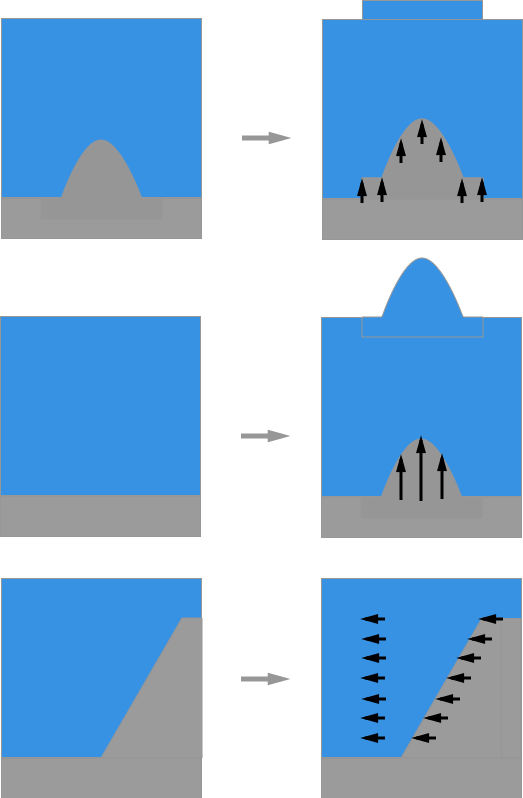
\includegraphics[width=0.8\textwidth]{earth_quake_tsunami_source.png}
    \end{center}
    \caption{Caption here}
    \label{fig:fault_movement_diagram}
\end{figure}

% ==============================================================================
%  Acknowledgments
\vskip 10pt
{\bf Acknowledgments.}


\bibliographystyle{plain}
\bibliography{database}

\end{document}